%! TEX program = lualatex
\documentclass[12pt,a4paper]{article} 

% Packages for formatting
\usepackage{fontspec}
\usepackage[ngerman]{babel}
\usepackage{geometry} 
\geometry{margin=1in} 
\usepackage{setspace} 
\usepackage{hyperref} 
\usepackage{xcolor}
\usepackage{amsmath} % for align*
\usepackage{amsthm} % neue Theorem-Umgebungen
\usepackage{enumitem} % für schöne Listen (Teilaufgaben)
\usepackage{mathbbol}
\usepackage{graphicx}
\usepackage{amssymb}
\usepackage{gensymb}

% Style settings
\pagecolor{darkgray}      % sets background color to black
\color{gray}          % sets text color to white

% Change subsection to use a, b, c instead of 1, 2, 3
\renewcommand{\thesubsection}{\alph{subsection})}

% Title page info 
\title{Blatt 08}
\author{Hannes Rall \\ Albert-Ludwigs-University}
\date{\today}

\begin{document}
% Title page 
\begin{titlepage}
    \centering
    \vspace*{2cm}
    {\Huge\itshape Blatt 08\par}
    \vspace{2cm}
    {\Large\textsc{Hannes Rall}\par}
    \vfill
    {\large Albert-Ludwigs-University\\}
    \vspace{1cm}
    {\large\today\par}
\end{titlepage}

\newpage
\section*{Aufgabe 22}
\subsection*{(i)}
Ich hab diese Aufgabe erst versucht anders zu lösen, bin aber gescheitert bzw an einer Stelle später die ich angemerkt habe nicht weitergekommen. Hier erst der richtige Beweis uns später der "Versuch". Wäre cool, wenn du den Versuch trotzdem korrigieren, aber nicht bewerten könntest. Eventuell weißt du auch die fehlende Begründung.\\
\\
Da die euklidische Gerade durch zwei Punkte $q$ und $r$ eine Sehne des Kreises ist, der die hyperbolische Gerade durch diese Punkte darstellt, gilt für die hyperbolischen Winkel $\beta$ und $\gamma$ im Vergleich zu den entsprechenden euklidischen Winkeln $\beta_E$ und $\gamma_E$:

\begin{align*}
    & \beta<\beta_E \\ 
    & \gamma < \gamma_E 
\end{align*}

\noindent In einem hyperbolischen Viereck können maximal zwei der vier Seiten teile einer euklidischen Geraden sein, zwei weitere müssen Halbkreise sein welche die hyperbolische Gerade darstellen (Wie sagt man das richtig?). Somit sind alle vier Winkel kleiner als ihr entsprechender euklidscher Winkel (Also dem der Sehne des Kreises). Da die Winkelsumme im euklidischen gleich $360^{\circ}$ ist, muss die Winkelsumme eines hyperbolischen Vierecks kleiner als $360^{\circ}$ sein. Daraus folgt direkt, dass es kein Rechteck in der hyperbolischen Ebene gibt. 

\newpage
\noindent Seien A, B, C und D verschiedene Punkte in $\mathbb{H}$.
\subsubsection*{1. Fall:}
Keine der Verbindungsgeraden der Punkte $A$, $B$, $C$, $D$ ist senkrecht zur $x$-Achse.

\begin{figure}[htbp]
    \centering
    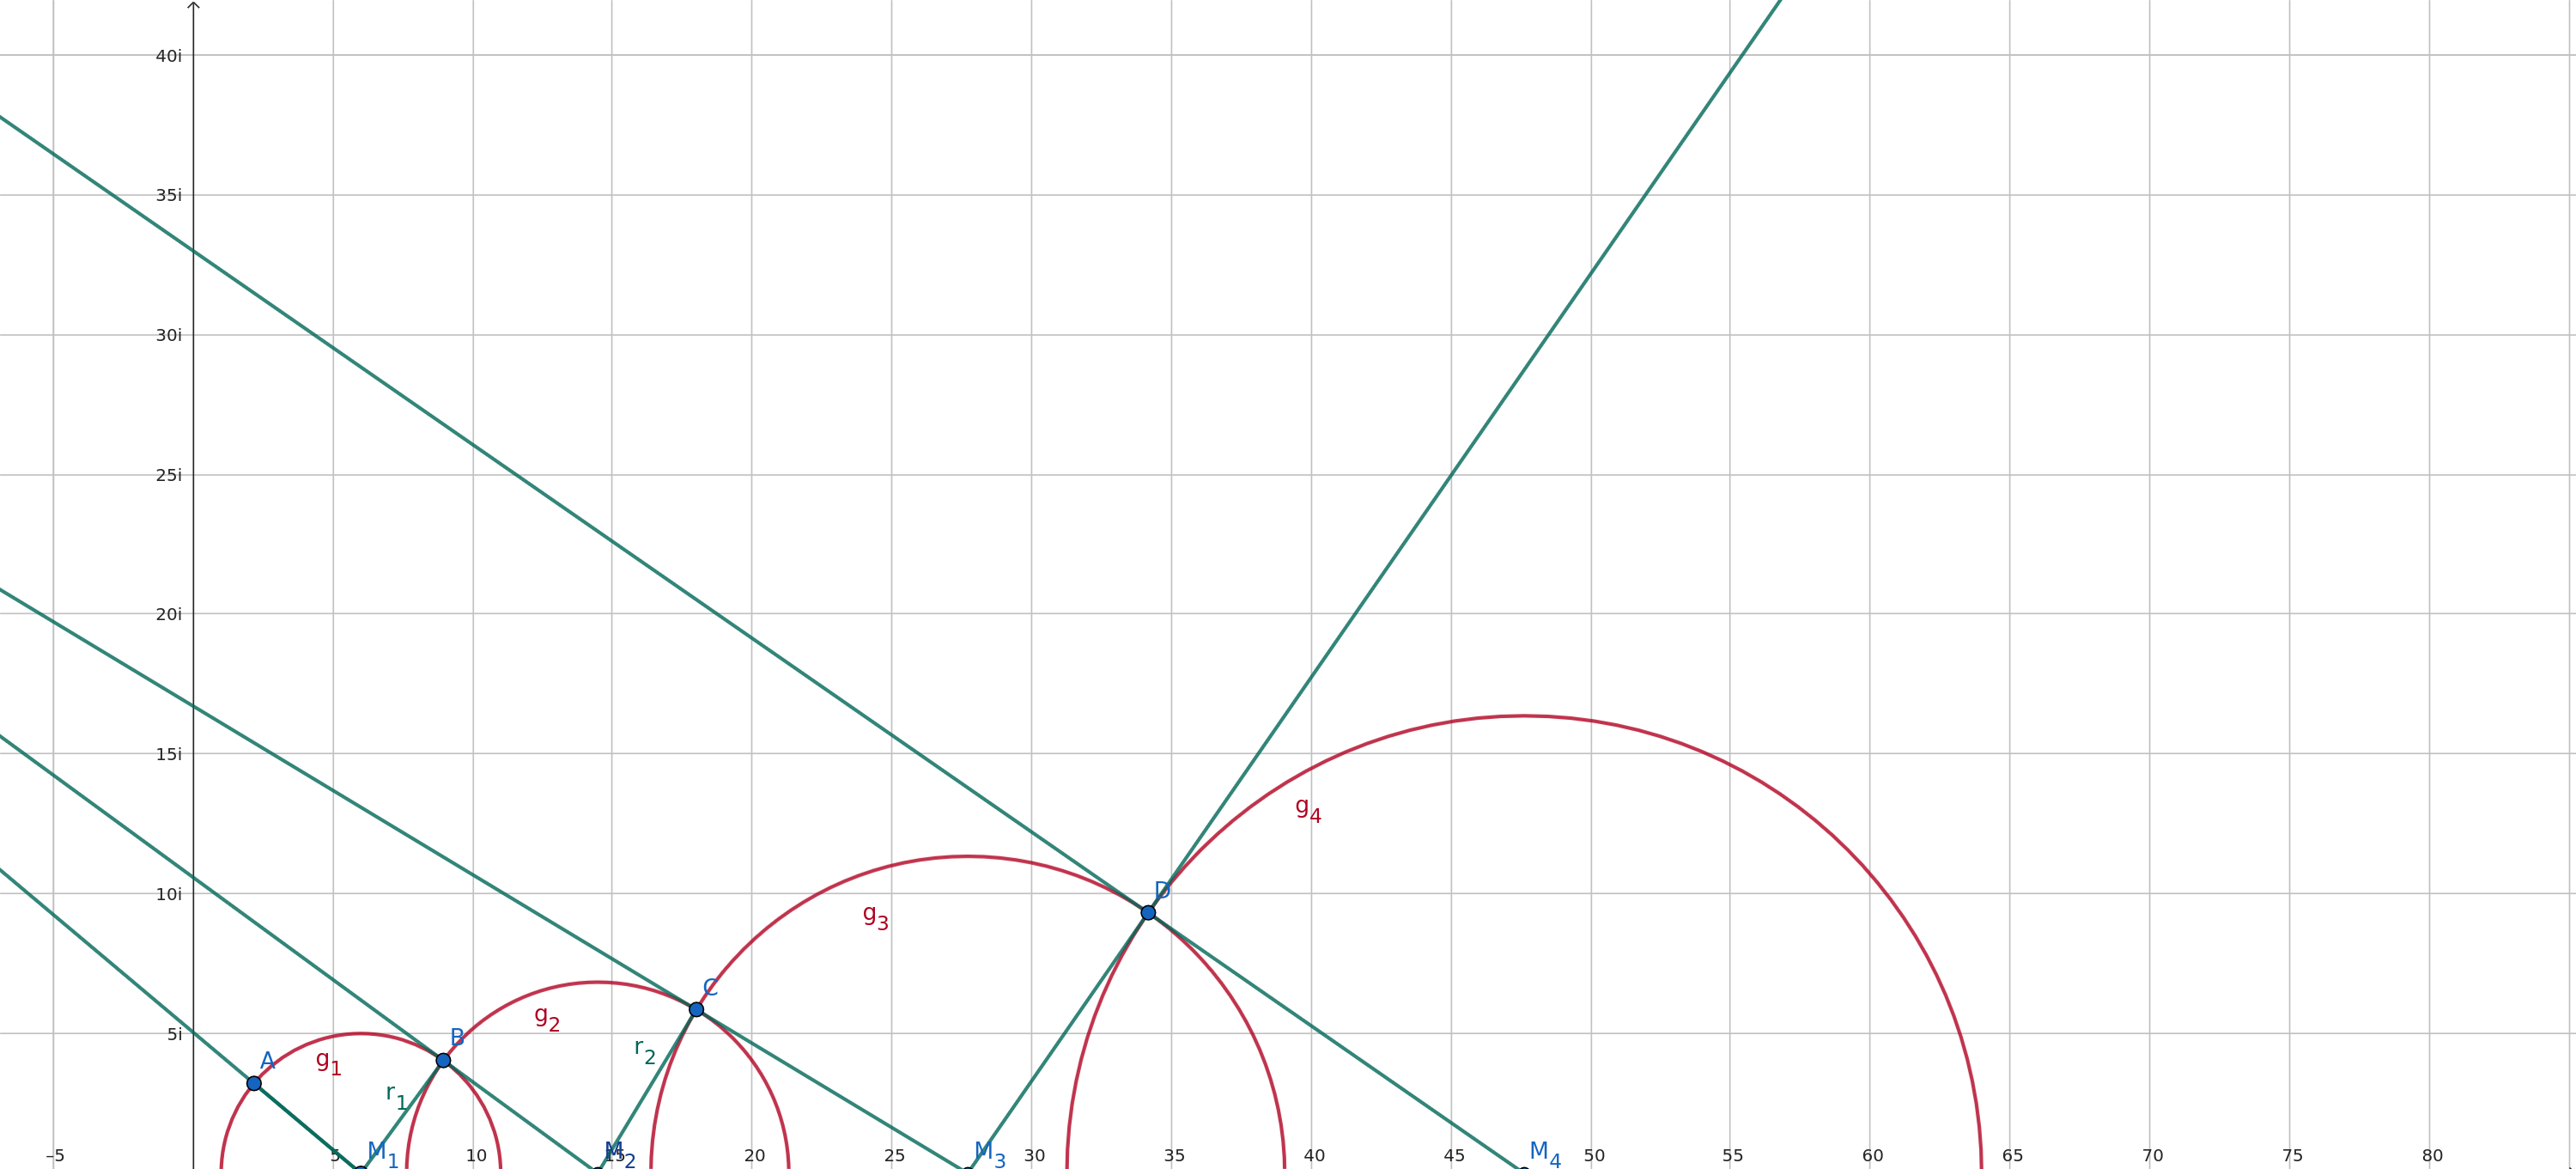
\includegraphics[width=0.8\textwidth]{Blatt08_Aufgabe_22_ia.png}
    \caption{1 Fall}
    \label{fig:Aufgabe_22_ia}
\end{figure}

\noindent Wir betrachten den Punkt $A$ und die zugehörige Gerade $g_1$ mit Mittelpunkt $M_1$ sowie die Tangente $t_{A_1}$ an $A$. Damit die nächste Gerade $g_2$ durch $A$ mit Mittelpunkt $M_2$ mit $g_1$ einen rechten Winkel einschließt, muss gelten: Der Schnittpunkt von $t_{A_1}$ mit der $x$-Achse ist identisch mit $M_2$ (da Tangeten senkrecht auf den Radius stehen). Wir wiederholen das Argument für die Gerade $g_3$. Wir haben also nun drei Geraden, wobei $g_1$ senkrecht auf $g_2$ steht und $g_2$ senkrecht auf $g_3$. Der Punkt D muss nun sowohl auf der Geraden $g_1$ als auch auf der Geraden $g_3$ liegen. Wenn D auf $g_3$ liegt, dann lässt sich das Tangentenargument wiederholen. Also der Schnittpunkt der Tangente durch D mit der $x$-Achse muss der Mittelpunkt von $g_4$ sein. Damit wiederum $g_4$ senkrecht auf $g_1$ steht, muss der Mittelpunkt $M_1$ der Schnittpunkt der Tangeten durch D mit der $x$-Achse sein. Jedoch ist die Tangente durch D gerade die Gerade durch D und $M_3$. Somit müssten $M_3$ und $M_1$ identisch sein, dann ist ABCD kein Vierreck mehr.

\newpage
\subsubsection*{2. Fall:}
Eine der Verbindungsgeraden der Punkte $A$, $B$, $C$, $D$ ist senkrecht zur $x$-Achse.

\begin{figure}[htbp]
    \centering
    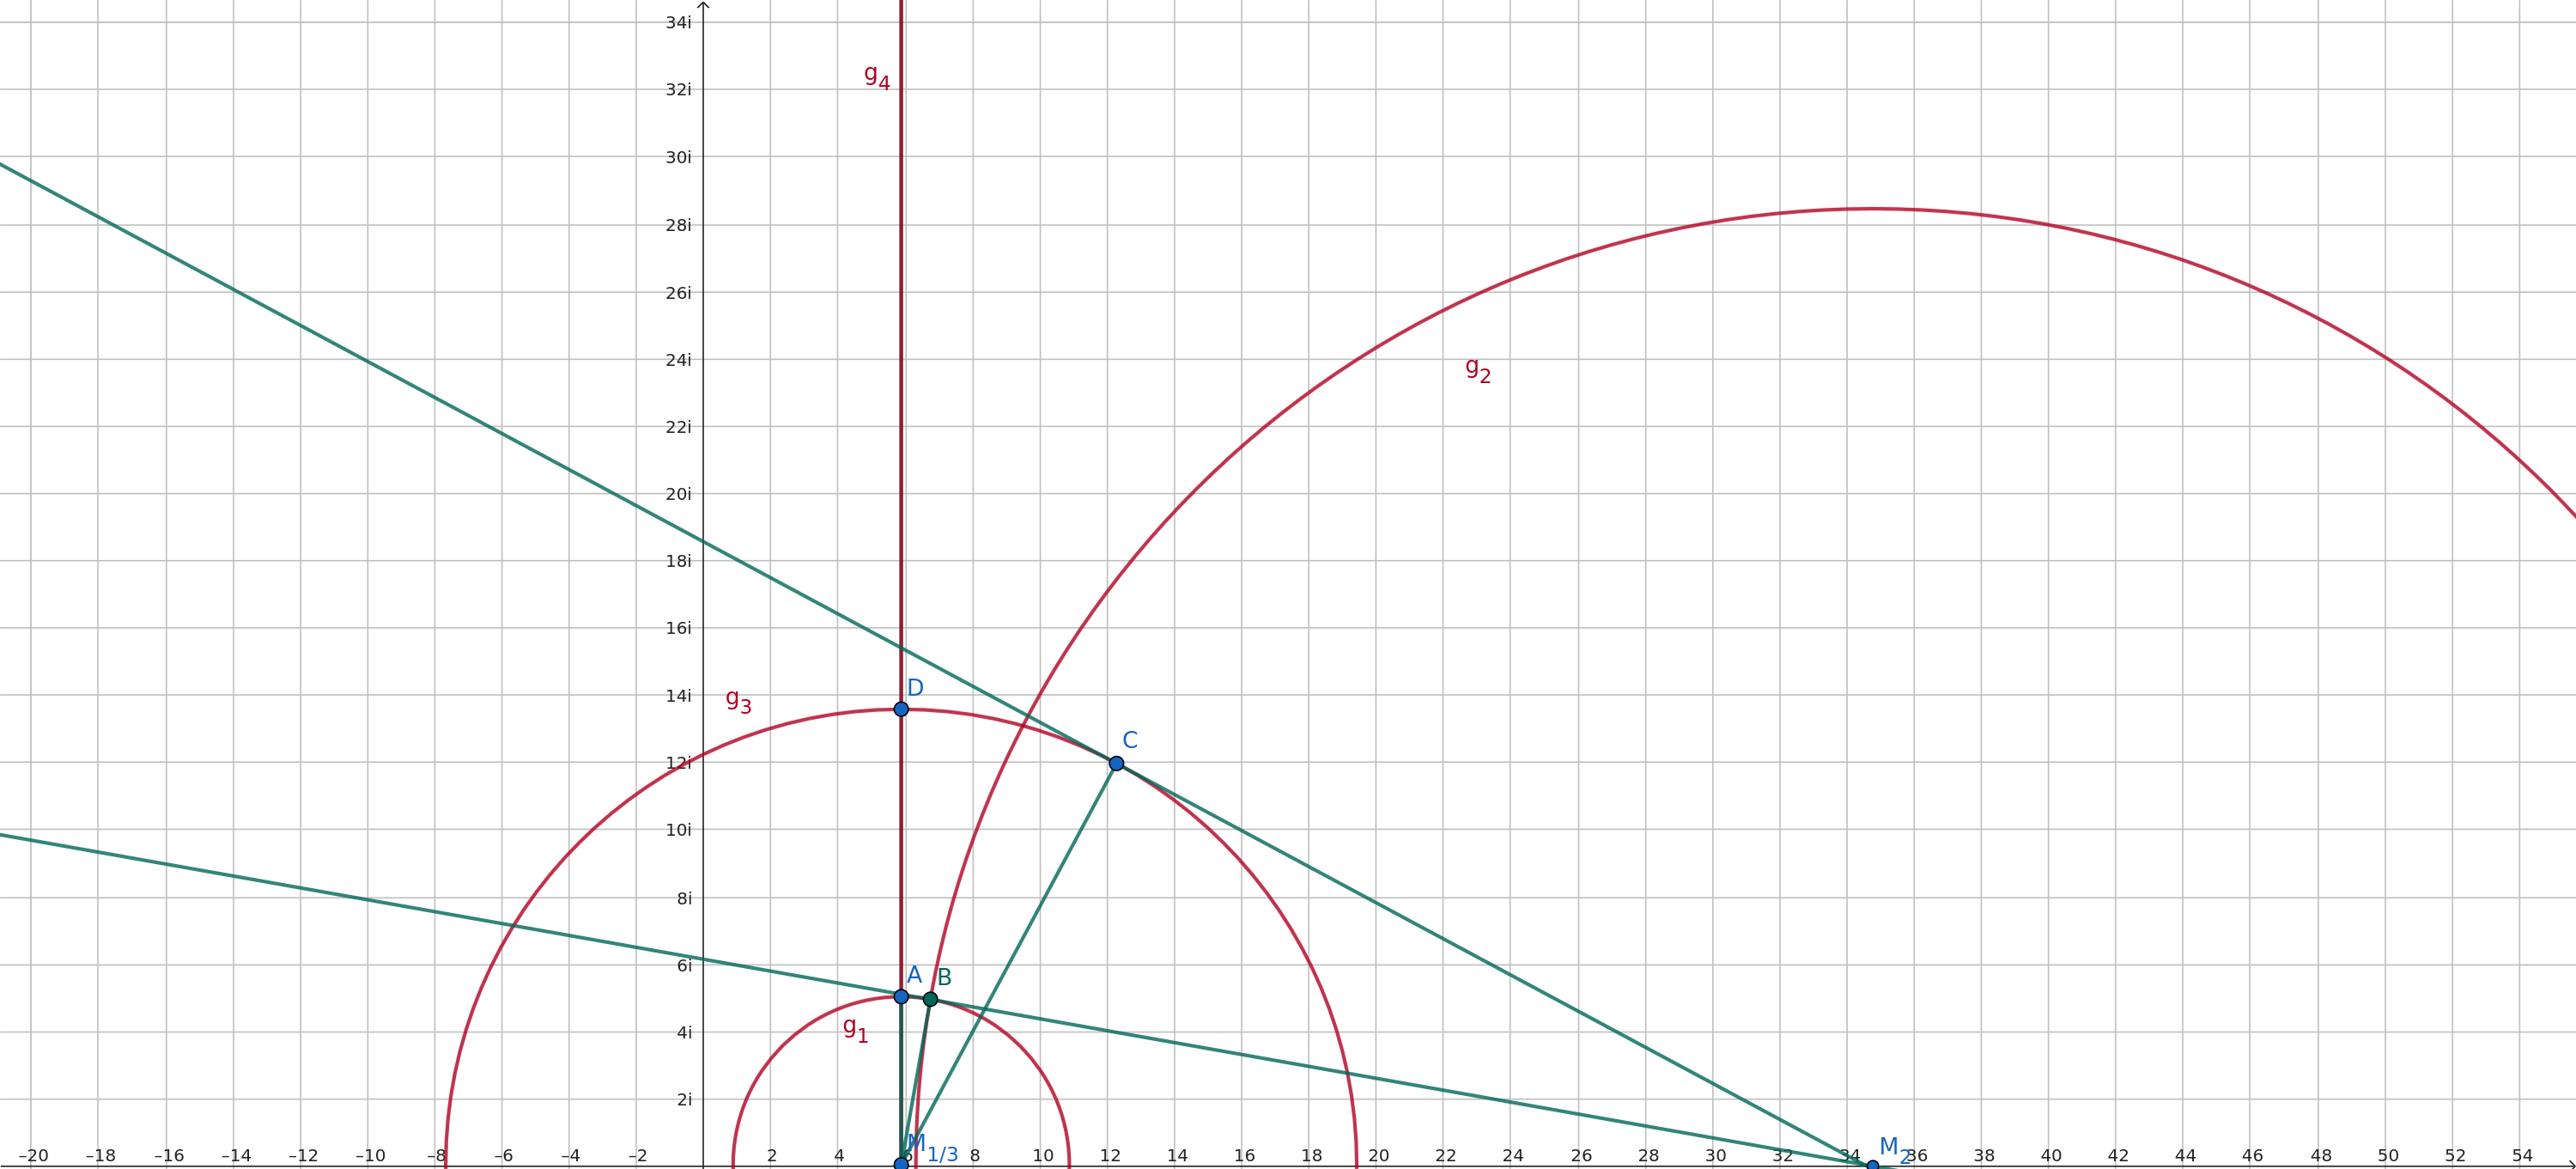
\includegraphics[width=0.8\textwidth]{Blatt08_Aufgabe_22_ib.png}
    \caption{2 Fall}
    \label{fig:Aufgabe_22_ib}
\end{figure}

\noindent Sei o.B.d.A. die Verbindungsgerade $g_4$ durch A und D senkrecht zur $x$-Achse. Die Verbindungsgerade $g_1$ durch A und B kann somit keine senkrechte Gerade zur $x$-Achse sein und lässt sich über Tangente eindeudtig bestimmen. Gleiches gilt für die Verbindungsgerade $g_3$ durch D und C, wobei $M_1 = M_3$ (Die Mittelpunkte der Geraden) sein muss. Wenn A und D verschieden sind, haben die Geraden $g_1$ und $g_3$ verschiedene Radien und die Gerade $g_2$ muss mit $g_1$ und mit $g_2$ einen gemeinsamen Punkt haben. Wenn $g_2$ senkrecht wäre, dann müsste die Tangente durch B an $g_1$ paralell zur $x$-Achse verlaufen. Das ist aber nur in A der Fall, dann wäre $A=B$ und ABCD kein Vierreck. Somit muss die Gerade $g_2$ einen Mittelpunkt auf der $x$-Achse haben und sowohl der Schnittpunkt der Tangente durch B and $g_1$ sein als auch der Schnittpunkt der Tangente durch C and $g_3$. Der Schnittpunkt einer Tangeten an einem Halbkreis mit der $x$-Achse liegt immer außerhalb des Halbkreises oder darauf, falls der Punkt an dem die Tangente angelegt ist selbst schon auf der $x$-Achse liegt, was wir ausgeschlossen haben, da sonst $g_2$ senkrecht auf der $x$-Achse stehen würde. Somit muss der Schnittpunkt der Tangente an B von $g_2$ auf der $x$-Achse liegen und "rechts" des Randes von $g_3$. (Hier weiß ich nicht die Begründung, aber dann rückt B immer näher an A heran der Halbkreis $g_2$ schneidet entweder die Gerade $g_3$ nicht mehr in C oder die Tangenten schneiden sich nicht mehr auf der $x$-Achse).

\newpage
\subsection*{(ii)}
Ich glaube ich mache hier einen Fehler. Das fühlt sich irgendwie falsch an.\\ 
Sei ein Pseudoquadrat ein Viereck in der hyperbolischen Ebene mit vier gleich langen Seiten mit der Länge a und vier gleichen Innenwinkeln $\gamma$. \\
Bezeichne die Ecken des Vierecks mit $A$, $B$, $C$, $D$ (in dieser Reihenfolge). Zerlegt man das Viereck entlang der Diagonalen $AC$ welche die Länge d hat, so entstehen zwei kongruente Dreiecke $ABC$ und $CDA$ (Nach SWS). In der hyperbolischen Geometrie gilt der Basiswinkelsatz samt Umkehrung: Ein Dreieck ist genau dann gleichschenklig, wenn es zwei gleiche Winkel besitzt. (Hinrichtung erhält man aus SWS und Rückrichtung aus WSW).
Im Dreieck $ABC$ (bzw $CDA$) gilt:
\begin{itemize}
    \item Der Winkel bei $B$ bzw $D$ ist der volle Innenwinkel $\gamma$ des Vierecks.
    \item Die Winkel bei $A$ und $C$ sind $\alpha$ (bzw. $\beta$) nach Basiswinkelsatz.
\end{itemize}
Nun muss nach dem Sinussatz für hyperbolische Dreiecke gelten:
\begin{align*}
    & \frac{sinh(a)}{sin(\alpha)} = \frac{sinh(a)}{sin(\gamma)} = \frac{sinh(d)}{sin(\gamma)}\\
    &\Leftrightarrow sin(\gamma)cos(\beta) - sin(\beta)cos(\gamma)= sin(\beta) \\
    &\Leftrightarrow (\sin(\alpha)\cos(\beta) + \sin(\beta)\cos(\alpha))\cos(\beta) - \sin(\beta)\left( \cos(\alpha)\cos(\beta) - \sin(\alpha)\sin(\beta) \right) = \sin(\beta) \\
    &\Leftrightarrow \sin(\alpha)\cos(\beta)^2 + \sin(\beta)\cos(\alpha)\cos(\beta) - \sin(\beta)\cos(\alpha)\cos(\beta) + \sin(\alpha)\sin(\beta)^2 = \sin(\beta)\\
    &\Leftrightarrow \sin(\alpha)(\cos(\beta)^2 + \sin(\beta)^2) = \sin(\beta) \\
    &\Leftrightarrow \sin(\alpha) = \sin(\beta)
\end{align*}

\noindent Und da sowohl $\alpha$ als auch $\beta$ kleiner als $\pi$ sein müssen aufgrund der Winkelsumme im Dreieck in der hyperbolischen Ebene, folgt direkt $\alpha = \beta$.\\
Nimmt man nun einen beliebigen Winkel $0 < \gamma < \frac{pi}{2}$ und einen beliebigen Punkt B durch den zwei Geraden gehen welche $\gamma$ einschließen, dann kann man ein gleischenkliges Dreieck konstruieren, in dem man für eine beliebige Länge entlang der zwei Geraden die Punkte A und C bestimmt. Nun bestimmt man die eindeutig bestimme Gerade durch A und C. Aufgrund des Basiswinkelsatzes sind dann dann die zwei Winkel bei A und C gleich. Nun gibt es genau ein kongruentes Dreieck CDA zu ABC welches man konstruieren kann und man hat das Pseudoquadrat. (Hier bei dem letzten Teil bin ich mir nicht sicher ob es dieses Pseudoquadrat wirklich immer geben muss).

\subsection*{(iii)}
Die hyperbolische Ebene kann mit Pseudoquadraten parkettiert werden, deren Innenwinkel
\[
\alpha = \frac{2\pi}{m}
\]
für ganze Zahlen \(m \geq 5\) beträgt. Nur für solche Winkel ist eine Parkettierung mit regelmäßigen Pseudoquadraten möglich, weil dann die Winkelsumme an jedem Knoten genau \(2\pi\) ergibt und die Winkelsumme des Vierecks kleiner als \(2\pi\) bleibt.

\newpage
\section*{Aufgabe 24}
\subsection*{(i)}
Die Charakterisierung der Mittelsenkrechten besagt: \\
Ein Punkt $P$ liegt genau dann auf der Mittelsenkrechten der Strecke $AB$, \\ 
wenn $d(PA) = d(PB)$ gilt.\\
Diese Aussage gilt auch in der hyperbolischen Geometrie, da dort ebenfalls die Distanzfunktion wohldefiniert ist und die Mittelsenkrechte als die Menge aller Punkte definiert ist, die von $A$ und $B$ denselben (hyperbolischen) Abstand haben.  
Für jeden Punkt $P$ in der hyperbolischen Ebene ist $|PA| = |PB|$ genau dann, wenn $P$ auf der Mittelsenkrechten von $AB$ liegt.

\subsection*{(ii)}
Angenommen, in einem hyperbolischen Dreieck $ABC$ schneiden sich die Mittelsenkrechten der Seiten $AB$ und $BC$ in einem Punkt $M$.  
Dann gilt nach (i): $|MA| = |MB|$ und $|MB| = |MC|$, also $|MA| = |MB| = |MC|$.  
Somit ist $M$ von allen drei Eckpunkten gleich weit entfernt.  
Nach (i) liegt $M$ damit auch auf der Mittelsenkrechten der dritten Seite $CA$.

\subsection*{(iii)}
Es gibt hyperbolische Dreiecke, bei denen die Mittelsenkrechten der Seiten keinen Schnittpunkt besitzen, die also keinen Umkreis haben. Es sei \( A := i \), \( B := 6 + i \) und \( C := 4i \). Dann gilt für die entsprechenden Mittelsenkrechten \( m_{AC} = K(0;2) \cap \mathbb{H} \) und \( m_{AB} = 3 + i\mathbb{R}_{>0} \). Offenbar besitzen \( m_{AB} \) und \( m_{AC} \) keinen Schnittpunkt.
\end{document}
